% 
\begin{figure}[!t]
    \centering
    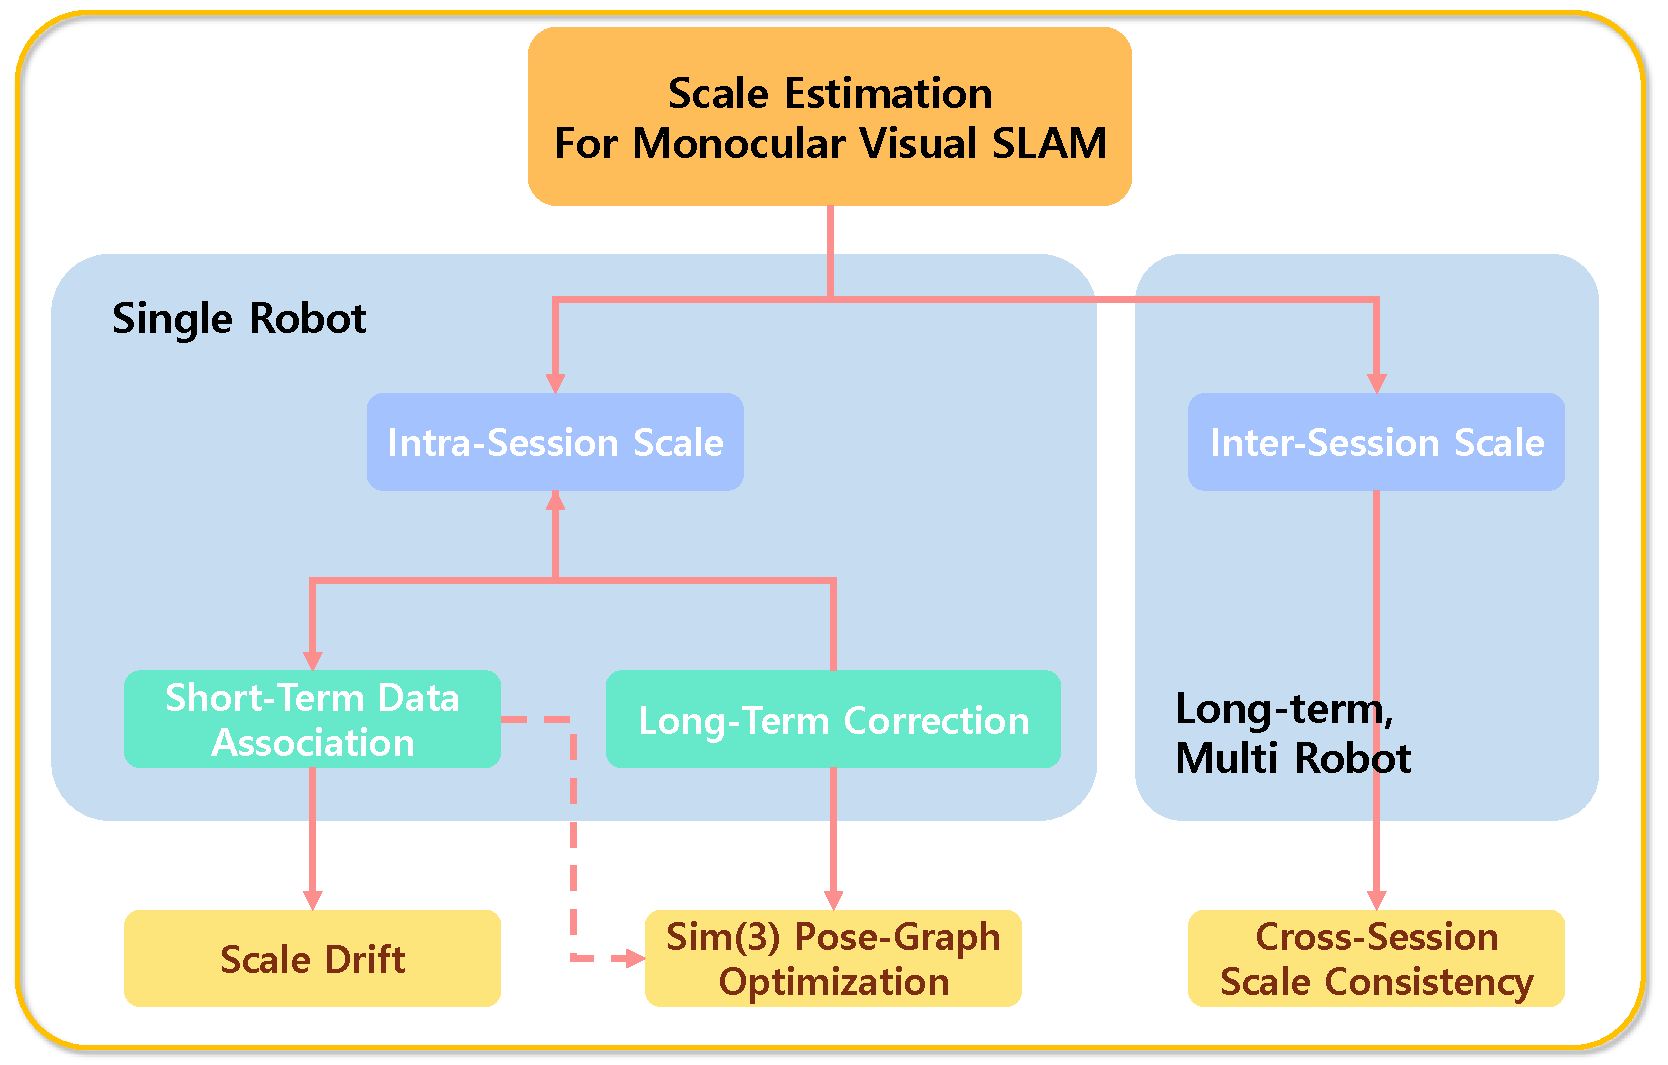
\includegraphics[width=0.98\columnwidth]{fig/fig2_resized.pdf}
    % 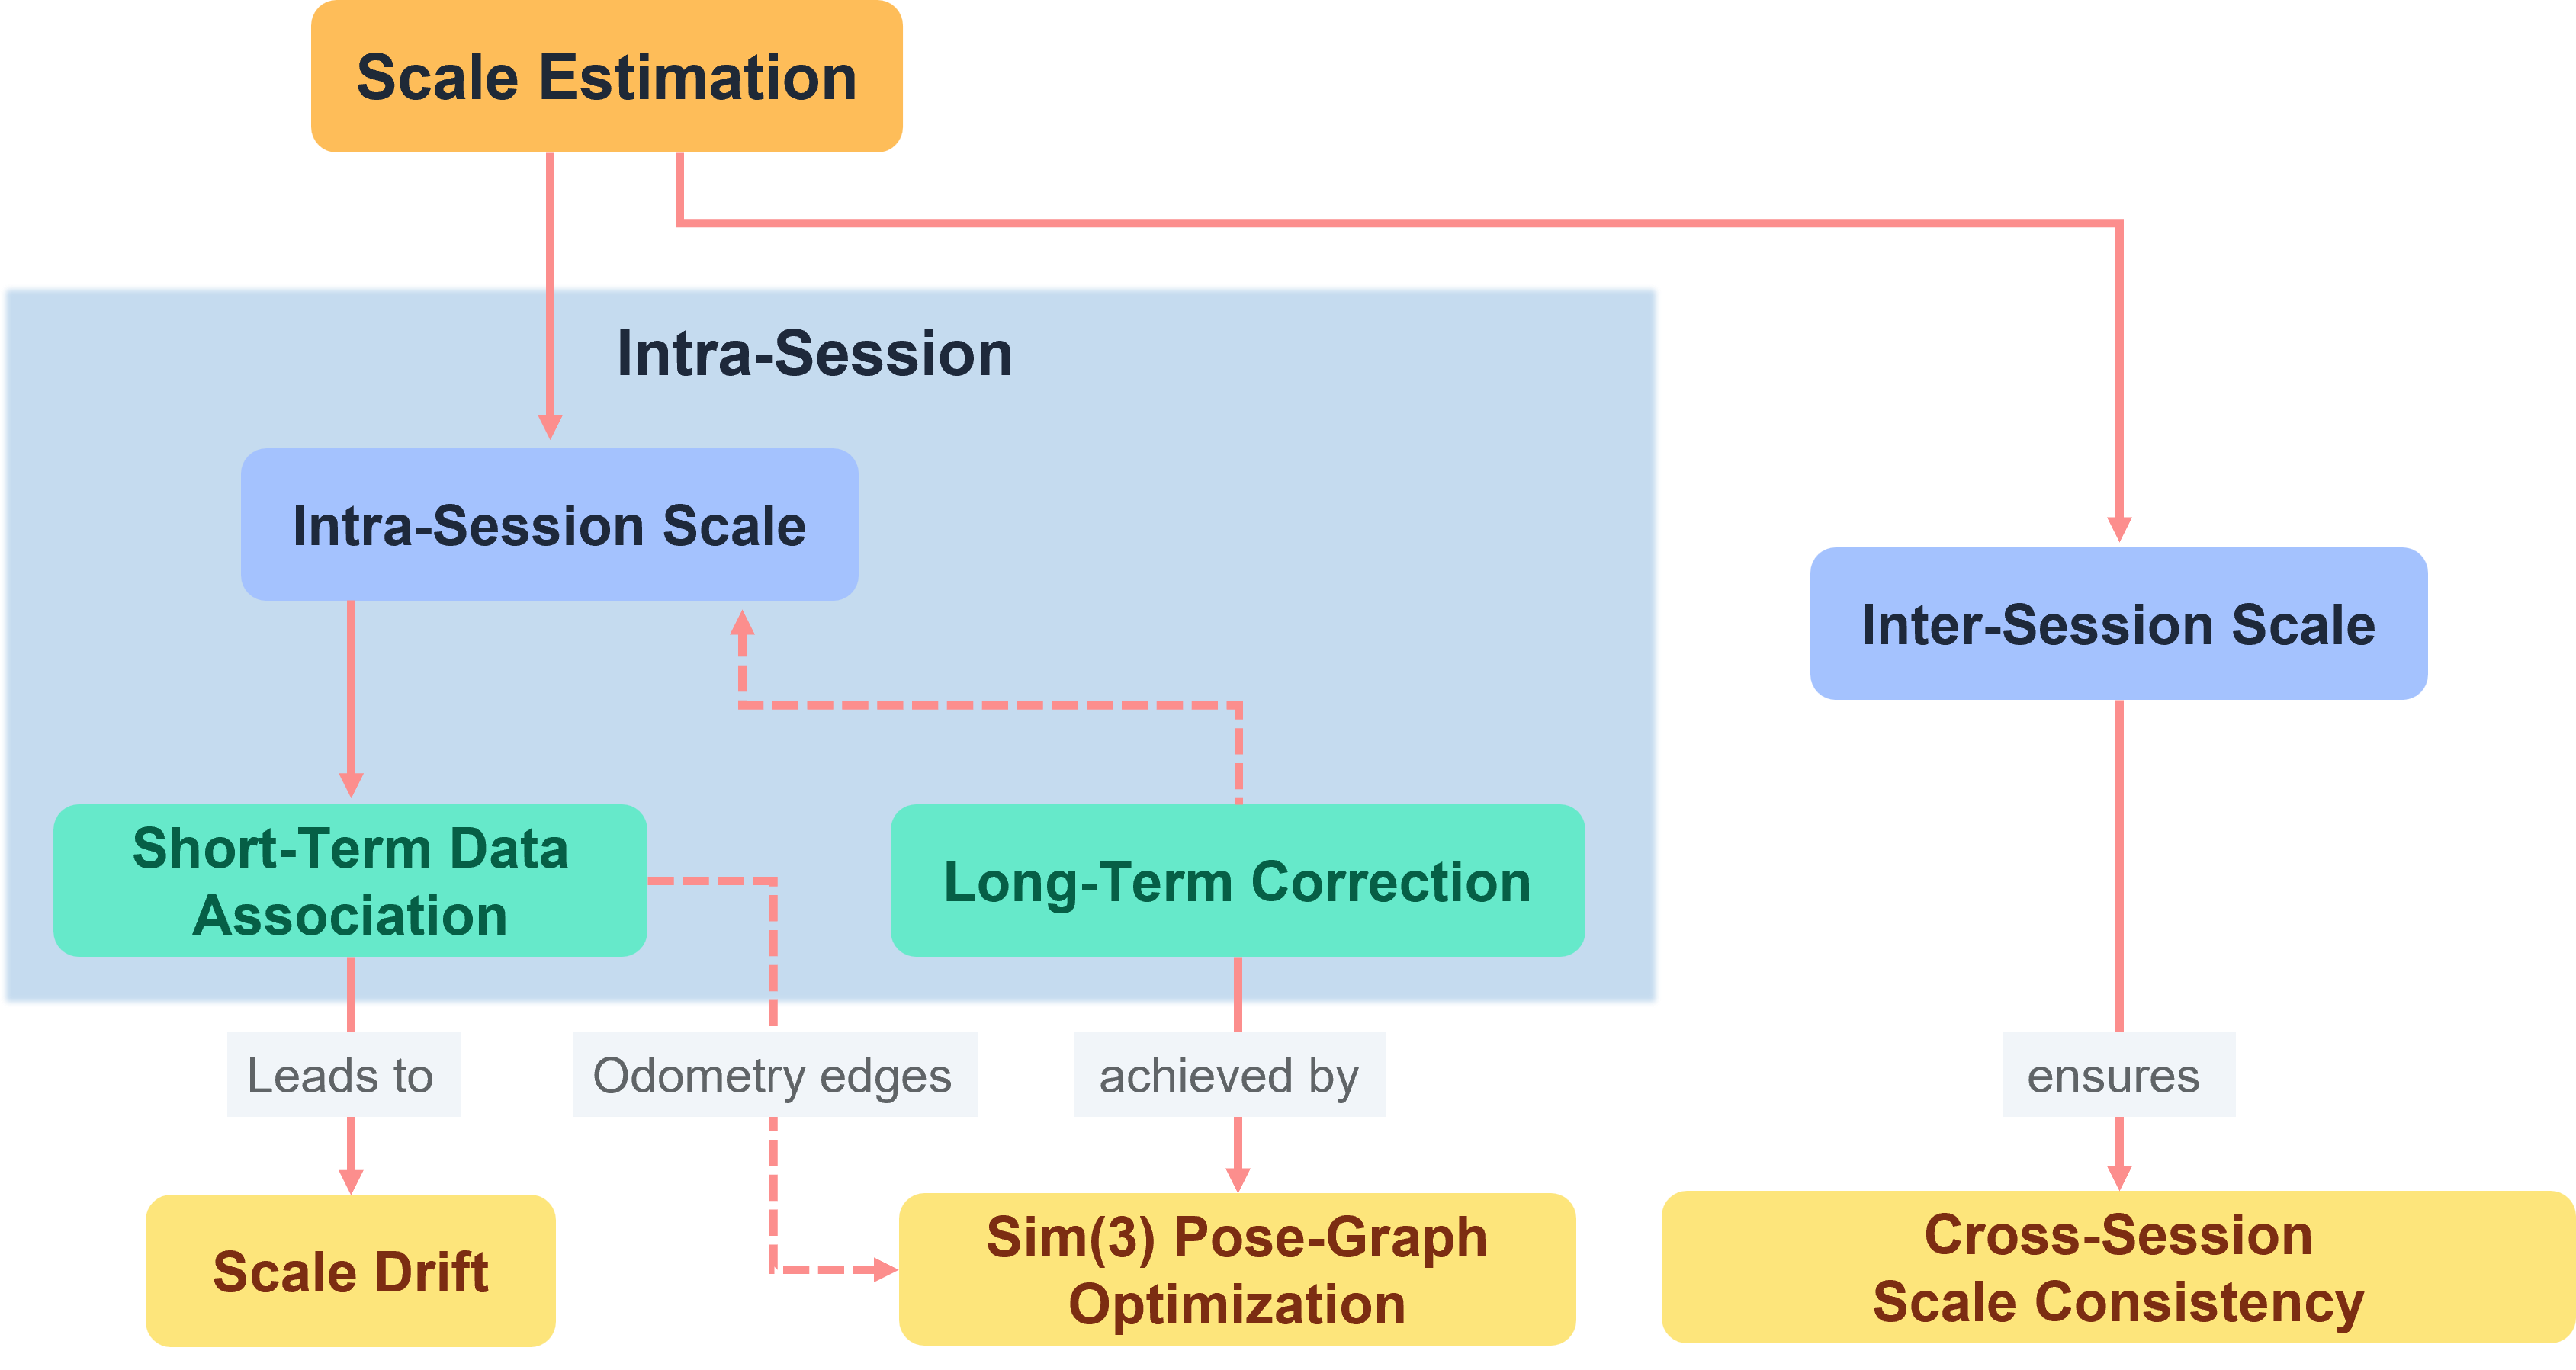
\includegraphics[width=10cm]{fig/r5.png}
    \caption{A diagram illustrating the components of the scale estimation problem.}

    \vspace{-3mm}
    
    \label{fig:problem_diagram}
\end{figure}
% 

%%%%%%%%%%%%%%%%%%%%%%%%%%%%%%%%%% 
\section{Problem Definition}
\label{sec:prob_def}

% 
\begin{table*}[!t]
\centering
\caption{\textbf{Comparison of public benchmark datasets with ours.}}
\resizebox{0.85\textwidth}{!}{%
\begin{tabular}{c|ccc|cccc}
\midrule
\textbf{Dataset} & \textbf{Sequences} & \textbf{\begin{tabular}[c]{@{}c@{}}Avg. \\ Length\end{tabular}} & \textbf{Image Resolution} & \textbf{\begin{tabular}[c]{@{}c@{}}Multi-floor \& \\ Elevation\end{tabular}} & \textbf{\begin{tabular}[c]{@{}c@{}}Pure \\ Rotation\end{tabular}} & \textbf{\begin{tabular}[c]{@{}c@{}}Complex \\ Indoor\end{tabular}} & \textbf{\begin{tabular}[c]{@{}c@{}}Scale Study \\ Feasibility\end{tabular}} \\ \midrule
\textbf{EuRoC} & 11 & 81.2 m & $752 \times 480$ & $\triangle$ & X & X & X \\
\textbf{TUM-RGBD} & $\sim$39 & 12.2 m & $640 \times 480$ & X & X & X & X \\
\textbf{7-Scenes} & 7 & 64.3 m & $640 \times 480$ & X & X & X & X \\
\textbf{ARKitScenes} & \textgreater 5,000 & \textless 100 m & $1920 \times 1440$ & X & O & X & X \\ \midrule
\textbf{Ours (ScaleMaster dataset)} & 25 & 152.2 m & $1920 \times 1440$ & O & O & O & O \\ \midrule
\end{tabular}
}
\label{dataset_comparison}
\end{table*}
% 

% 
\begin{figure*}[t]
    \centering
    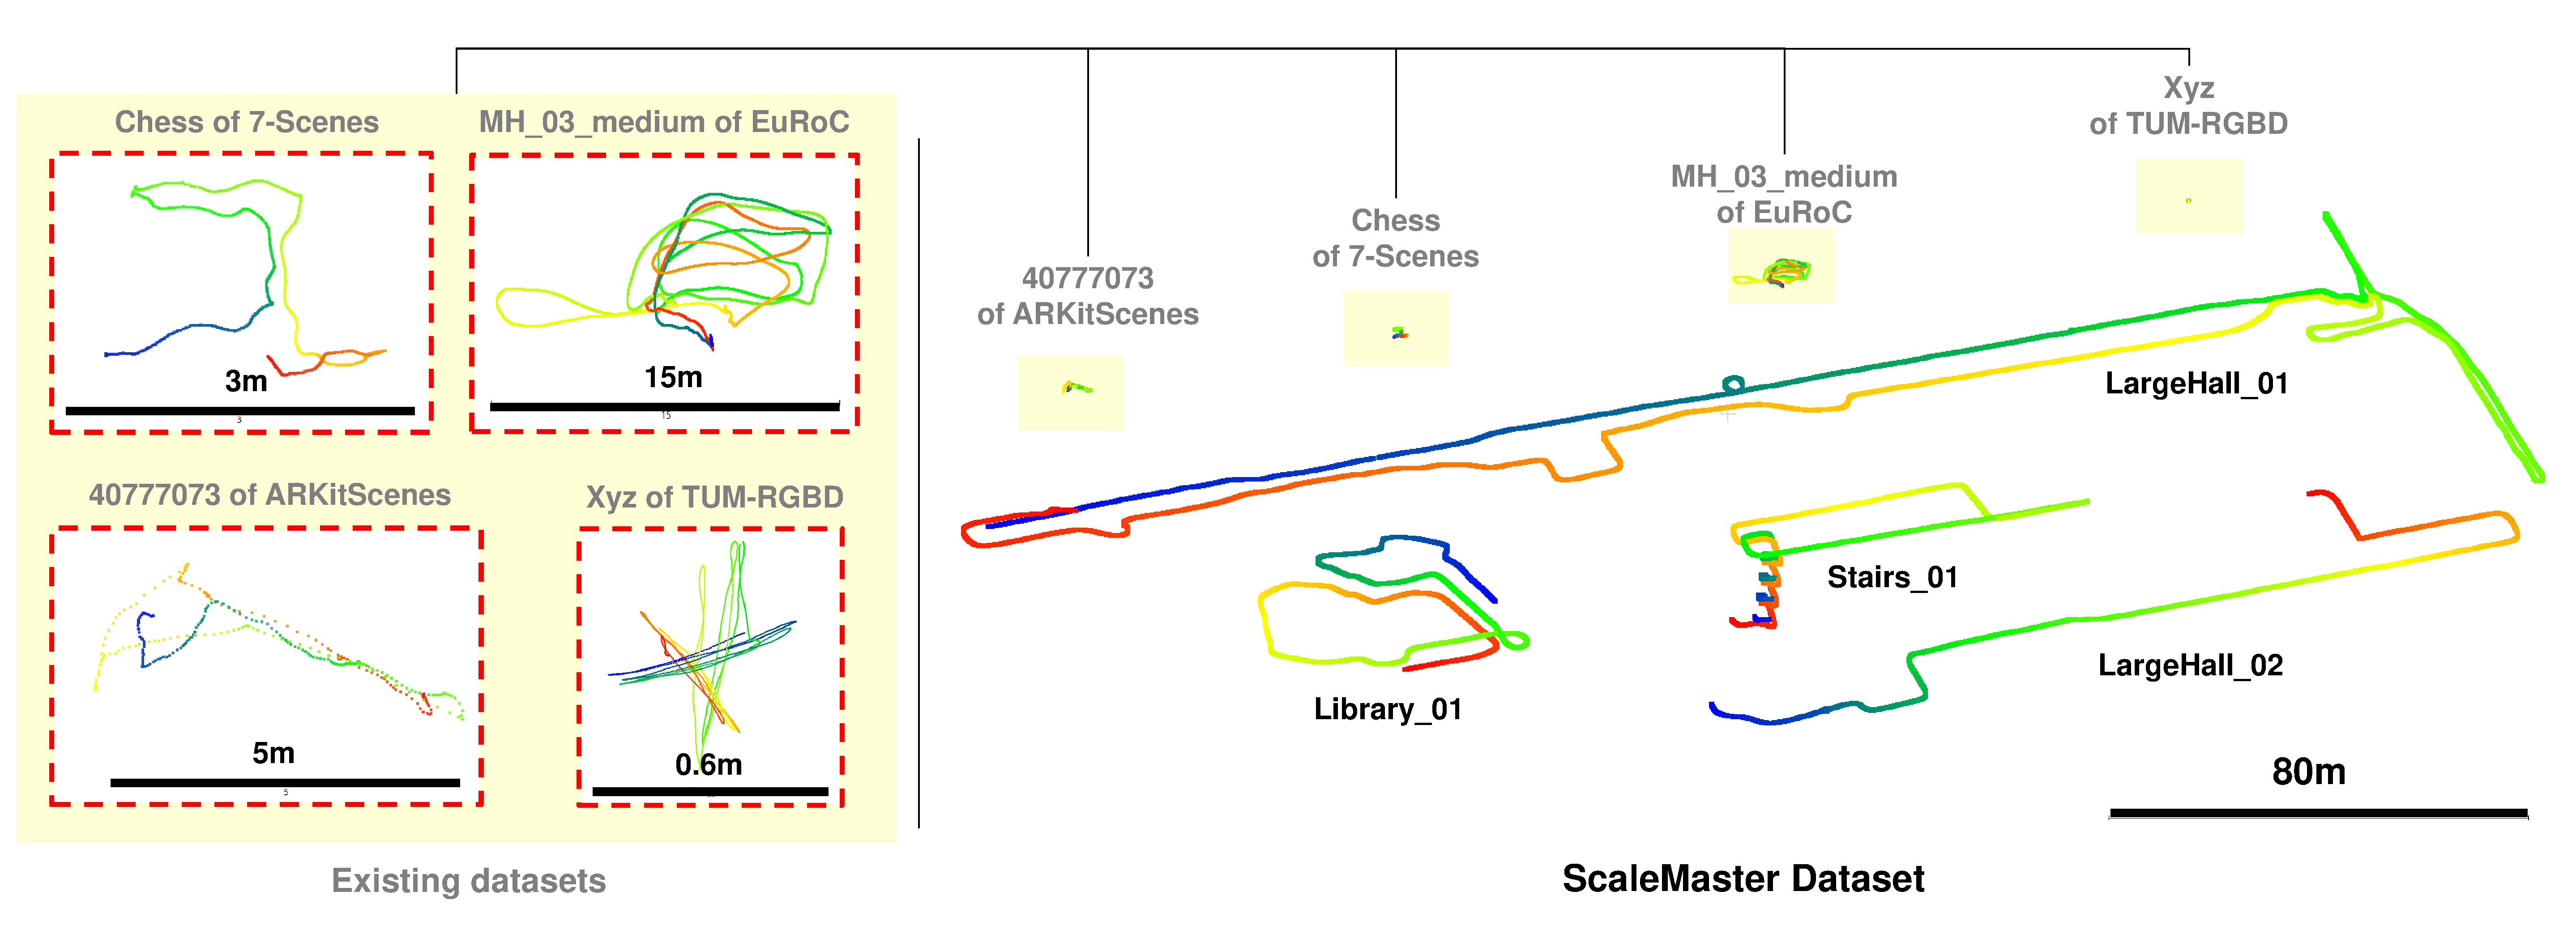
\includegraphics[width=0.98\textwidth]{fig/fig_scalemaster_traj_v3.pdf}
    \caption{A visual comparison of trajectory scales between our proposed ScaleMaster dataset and existing standard benchmarks. This distinct contrast visually demonstrates why existing room-scale benchmarks are insufficient for evaluating long-term scale consistency failures.}
    \label{fig:trajectory_comparison}

    \vspace{-3mm}

\end{figure*}
% 

The scale consistency problem in monocular visual \ac{SLAM} can be categorized into two primary challenges as in \figref{fig:problem_diagram}: Intra-session inconsistency, which occurs within a single run, and inter-session ambiguity, which arises between multiple runs (e.g., long-term map management or multi-robot collaborative mapping). 

\subsection{Intra-Session Scale Inconsistency}
Intra-session scale inconsistency refers to the scale errors that accumulate during a single \ac{SLAM} session. This problem arises primarily from the interplay of the following two factors:

\begin{itemize}    
    \item \textbf{Short-Term Data Association \& Scale Drift:} 
     Short-term data association establishes odometry edges by relating consecutive image frames. Due to the inherent unobservability of metric scale in monocular visual SLAM, relative scale drift inevitably arises between them \cite{hartley2003multiple}.

    \item \textbf{Long-Term Correction \& Limitations of $\text{Sim}(3)$ \ac{PGO}:} 
    Owing to the $\text{Sim}(3)$ gauge in monocular visual SLAM, scale cannot be fixed by $\text{SE}(3)$ optimization \cite{strasdat2010scale}; while $\text{Sim}(3)$ pose-graph optimization is standard, its small, Gaussian-error assumption makes it brittle to large, discontinuous loop-closure errors, leaving residual scale inconsistency.
    
\end{itemize}

% 
\subsection{Inter-Session Scale Ambiguity}
\label{sec:intersessionscale}
Inter-session scale ambiguity arises when attempting to merge multiple maps generated at different times or when trying to re-localize within a map from a previous session \cite{kim2010multiple}. If each session already contains its own unique and uncorrected scale drift, determining the relative scale between these maps becomes an extremely challenging problem. This ultimately leads to the failure of \textbf{Cross-Session Scale Consistency}, making it impossible to integrate multiple maps into a single, globally consistent representation.


% 
\renewcommand{\arraystretch}{1.2}
\begin{table*}[t]
\centering
\caption{\textbf{Summary of collected sequences and their characteristics.}}
\begin{threeparttable}
\resizebox{0.98\textwidth}{!}{%
\begin{tabular}{lccc p{5.5cm} p{4.2cm}}
\midrule
\textbf{Sequence Name} & \textbf{Frames} & \textbf{Path Length (m)} & \textbf{Duration (s)} & \textbf{Environment} & \textbf{Tags} \\ \midrule
\textbf{Basement\_01}   & 2036  & 29.11  & 67  & Basement area followed by a staircase ascent. & Indoor, Short trajectory, 3D Map \\
\textbf{HotelRoom\_01}  & 4217  & 29.07  & 141 & Interior traversal of a hotel room. & Indoor, Repetitive view, Short trajectory \\
\textbf{Lab\_01}         & 2167  & 25.85  & 72  & In-place rotations inside a lab room. & Indoor, Repetitive view, Short trajectory \\
\textbf{LargeHall\_01}  & 22830 & 884.12 & 761 & Full loop covering the entire LargeHall. & Indoor, Very long trajectory \\
\textbf{LargeHall\_02}  & 6576  & 241.89 & 219 & Evening traversal of a large open hall, low-light. & Indoor, Long trajectory, 3D Map \\
\textbf{LargeHall\_03}  & 2764  & 109.89 & 92  & Short loop inside the LargeHall at night. & Indoor, Low-texture risk, Medium trajectory \\
\textbf{LargeHall\_04}  & 4331  & 179.69 & 144 & Loop around the E1 section of LargeHall. & Indoor, Medium trajectory \\
\textbf{LargeHall\_05}  & 1912  & 54.21  & 63  & Traversal under low-light conditions. & Indoor, Short trajectory, 3D Map \\
\textbf{Library\_01}    & 6515  & 254.98 & 217 & Multi-floor descent from 5F to 3F with loops per floor. & Indoor, Long trajectory, Repetitive view, 3D Map \\
\textbf{Library\_02}    & 5001  & 163.58 & 166 & Single-floor loop on 4F with repetitive bookshelves. & Indoor, Medium trajectory, 3D Map \\
\textbf{Library\_03}    & 3136  & 105.81 & 105 & Loop on the 3rd floor of the library. & Indoor, Medium trajectory \\
\textbf{Library\_04}    & 5450  & 146.22 & 182 & Walking paths between library bookshelves. & Indoor, Repetitive view, Medium trajectory \\
\textbf{Library\_05}    & 2540  & 78.24  & 85  & Large open central atrium (depth sensor limitation). & Indoor, Low-texture risk, Short trajectory \\
\textbf{Library\_06}    & 2026  & 13.27  & 67  & 360-degree in-place rotation at the library center. & Indoor, Short trajectory, 3D Map \\
\textbf{Library\_07}    & 1580  & 5.23   & 52  & Static panoramic survey from the 1st floor. & Indoor, Short trajectory, 3D Map \\
\textbf{Library\_08}    & 2241  & 3.51   & 75  & Short traversal around the open central viewpoint. & Indoor, Low-texture risk, Short trajectory \\
\textbf{Library\_09}    & 2303  & 20.65  & 77  & In-place rotation in front of a 3F glass room. & Indoor, Repetitive view, Short trajectory \\
\textbf{Lobby\_01}      & 2893  & 104.83 & 96  & Traversal inside a lobby. & Indoor, Medium trajectory \\
\textbf{Lounge\_01}     & 6823  & 199.09 & 228 & Loop trajectory inside a lounge area. & Indoor, Medium trajectory \\
\textbf{Office\_01}     & 6009  & 154.50 & 200 & Traversal inside a repetitive office view. & Indoor, Repetitive view, Medium trajectory \\
\textbf{Parking\_01}    & 8218  & 323.01 & 274 & Full loop inside the underground parking lot (B2). & Underground, Long trajectory \\
\textbf{Parking\_02}    & 2270  & 88.06  & 76  & Loop in an indoor parking area. & Indoor, Short trajectory \\
\textbf{Stairs\_01}     & 9394  & 298.42 & 313 & Ascending from 2F to 6F, then looping on 6F. & Indoor, Vertical motion, Repetitive view, Long trajectory \\
\textbf{Stairs\_02}     & 4143  & 122.23 & 139 & Repeated ascending and descending of stairs. & Indoor, Vertical motion, Repetitive view, Medium trajectory \\
\textbf{Station\_01}    & 1715  & 170.84 & 229 & Escalator traversal inside a train station. & Indoor/Outdoor, Vertical motion, Repetitive view, Medium trajectory \\
\midrule
\end{tabular}
}% end resizebox
\begin{tablenotes}[flushleft]
\item \footnotesize Trajectory length tags : 0--100\,m = Short;\; 100--200\,m = Medium;\; $>$ 200\,m = Long.
\end{tablenotes}
\vspace{-3mm}
\end{threeparttable}
\label{dataset_summary}
\end{table*}
% 

% 
\begin{figure*}[t]
    \centering
    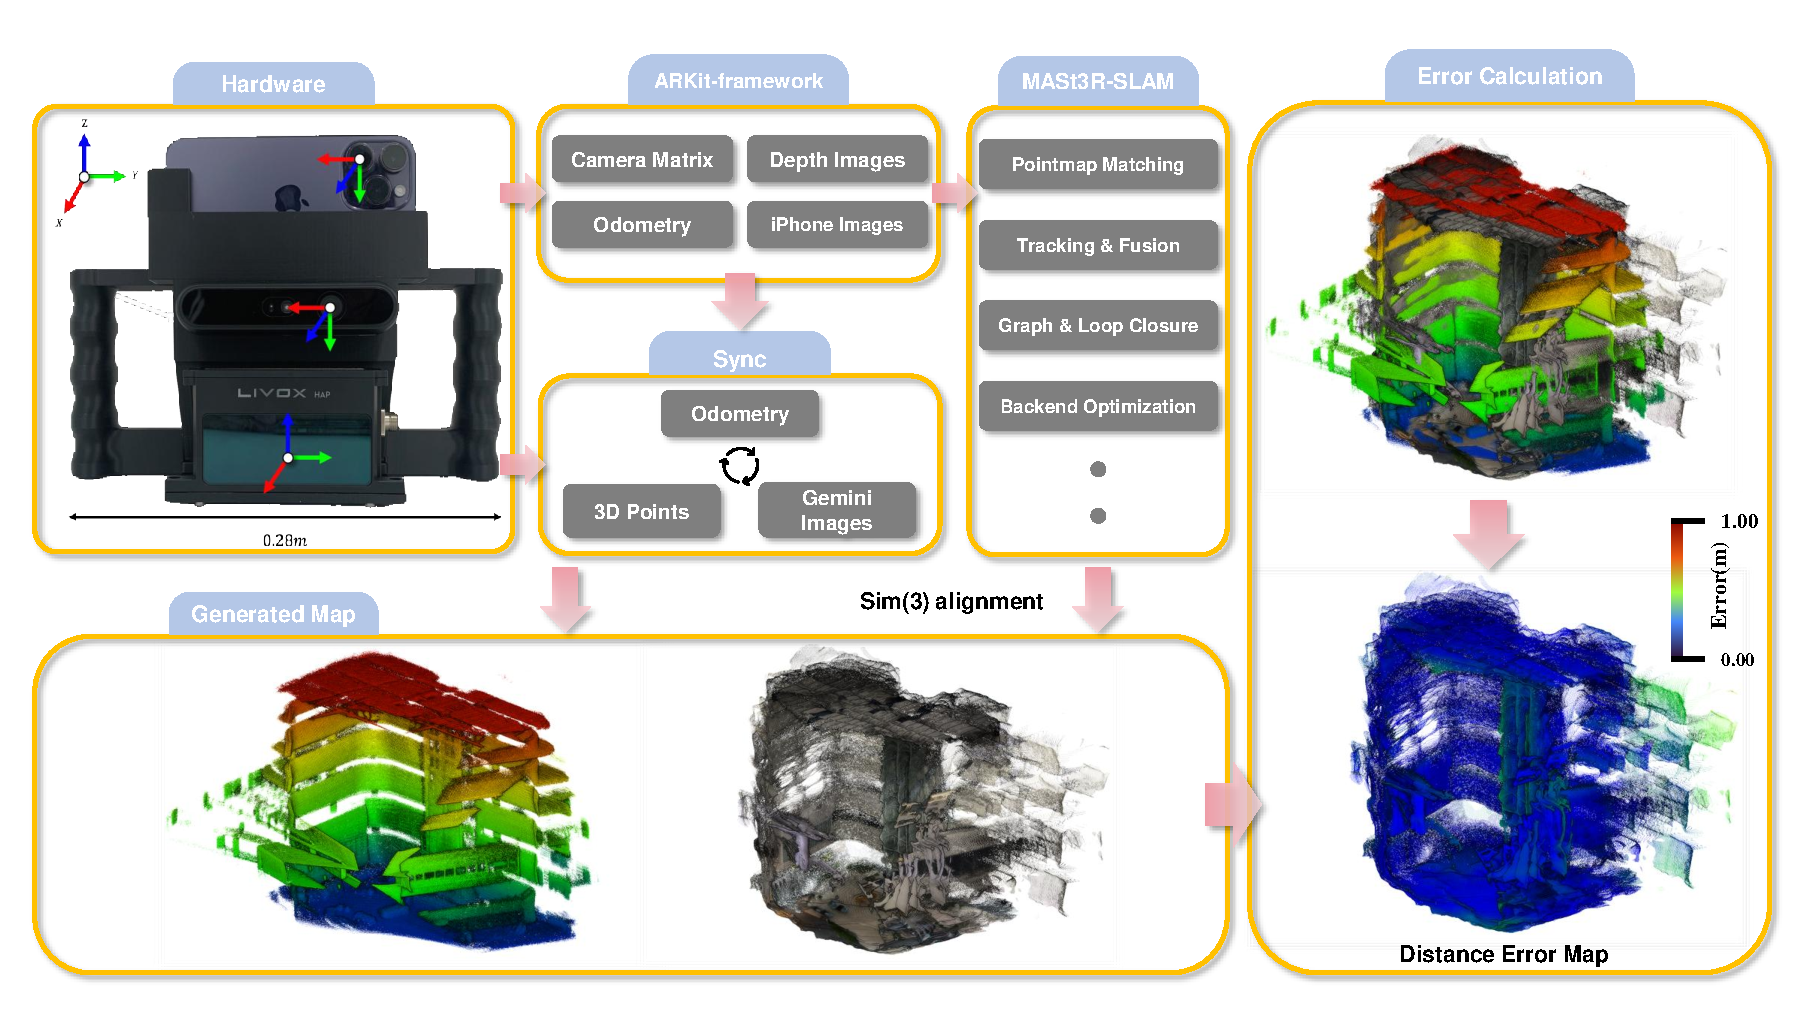
\includegraphics[width=0.9\textwidth]{fig/fig4_resized.pdf}
    \caption{Our overall experimental pipeline, illustrating the process from data acquisition with our custom rig (left), through ground truth map generation and SLAM processing (center), to the final map-to-map error calculation (right).}

    \vspace{-3mm}
    
    \label{fig:system_overview}
\end{figure*}
% 

In conclusion, this research critically addresses the challenges of intra-session scale drift and inter-session scale ambiguity, which are rooted in the fundamental scale ambiguity of monocular visual SLAM systems.
